\chapter*{Abstract}

\chapter{Introduction}
	The design process for a facility like a fusion power plant takes into account a manifold of aspects. Thereunder a cost analysis for the fusion device. To make an estimate of the cost analysis one has to consider the lifetime of machine parts. Most prominently the divertor and first wall suffer from shortened life spans due to erosion. Which is partly due to neutral particle induced sputtering.\\
	To include considerations like these in the design of a power plant one uses so called systems codes like PROCESS\cite{process}. These codes focus on optimizing design parameters of large scale systems like power plants, which consist of many smaller subsystems. Due to the amount of subsystems the need arises to simplify models in order to achieve reasonable run times for systems codes. The following work is concerned with deducing a fast surrogate in place of a simulation for the sputtering rate of a fusion device component.\\
	The following chapter gives a brief overview of the motivating applications while also introducing the concept of reduced model approaches via machine learning algorithms. Furthermore it considers which methods are most applicable in the given situation.\\
	
	\section{Fusion Devices}
	
	\begin{figure}[ht]
	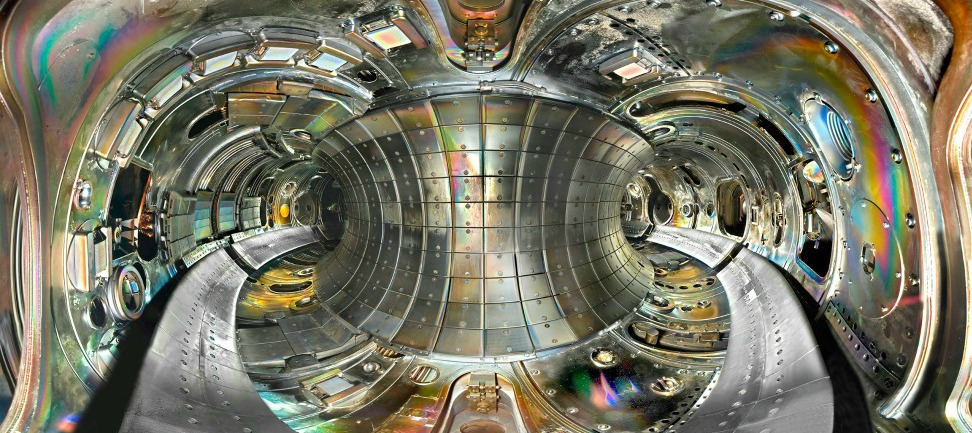
\includegraphics[width=\textwidth]{images/TEXTOR_tokamak_narrow.jpg}
	\caption{A picture of the TEXTOR Tokamak reactor. Depicting the inside with a wide angle camera shot.}
	\label{TEXTOR_JPG}
	\end{figure}
	
	Fusion technology has been an ongoing field of research for almost one century. The earliest records of fusion research go back to the 1920s when Francis William Aston discovered the potential energy gain of combining hydrogen atoms into helium atoms. Later in the 1920s Arthur Stanley Eddington proposed the proton-proton chain reaction as the primary working mechanism of the sun.\todo{add citation}\\
	The basic idea of fusion power generation is exploiting a difference in binding energy of different elements. A basic calculation as in \ref{eq_basic_fusion} shows that by combining the hydrogen isotopes deuterium and tritium into helium a neutron with $14.1$\.MeV is released which can be used to extract energy as heat, thus allowing fusion to be used as a means of generating electric power.
	\begin{equation}
		{}^2_1\textrm{D} + {}^3_1\textrm{T} \Rightarrow {}^4_2\textrm{He} (3.5\,\textrm{MeV}) + \textrm{n} (14.1\,\textrm{MeV})
		\label{eq_basic_fusion}
	\end{equation}\todo{maybe replace ${}^1_1$ with mathtools and \.MeV with units}
	The containment principle for fusion plasma is based on the magnetic bottle/mirror phenomenon.\todo{add citation} This allows to encase charged particles inside a magnetic field\todo{Add footnote and/or citation}. Neutral particles will not be confined by the magnetic field and quickly exit the fusion plasma towards the first wall of any fusion device. The impact of neutral particles will also lead to erosion of the wall.\\
	To counter the erosion of integral machine parts a device called blanket is used as a replaceable first layer. The operating life of the blanket needs to be taken into consideration for maintenance cycles and operating cost of a fusion power plant.
	
	\section{PROCESS Systems Code}
	The systems code PROCESS\cite{process} is concerned with the combination of physics, engineering and economical simulation and evaluation for a fusion power plant scenario\footnote{So far most published work has been on ITER and DEMO Tokamak like scenarios.}. It is based on TETRA (Tokamak Engineering Test Reactor Analysis) \cite{TETRA} and has been used for the Power Plant Conceptual Study \cite{PPCS}.\\
	
	PROCESS can be operated in two different modes, namely optimization mode and non-optimization mode. In non-optimization mode PROCESS will find a single set of parameters for ...\todo{formulate the extend of found parameters.}, while the more commonly used optimization mode finds a set of parameters that minimize or maximize a chosen figure of merit. The list of figures of merit includes capital cost, cost of electricity or more physical/engineering related quantities such as neutron wall load. Both modes result in a set of parameters consistent with the input parameters and constraints.\\ %Furthermore optimization mode will enforce inequalities in addition to the consistency equations which are also enforced in non-optimization mode
	There are several hundred input parameters which can be chosen as iteration variable for a run in optimization mode. Studies of a given design for a fusion device might want to use the optimization mode to scan a range in multiple input parameters, easily resulting in a high number of runs and an accordingly high total run time. Hence underlying physical models have to be sufficiently simplified in an attempt to balance required runtime against a higher potential for error.\\
	
	Further information on the details of PROCESS code operation can be found in the publication of M. Kovari et. al \cite{process}\todo{Fix citation}.\\
	
	\section{Reduced Model Approaches}
	Simulations based on complex models face the barrier of having long run times, which is often unsuited for studying general systematic behaviours. Reducing run time of numerical simulations can be achieved via model order reduction methods like dimensionality reductions.
	\todo{Read Model Order Reduction: Theory, Research Aspects and Applications by Wilhelmus H. A. Schilders}
	Ideally one would apply control theory to the given system with proper orthogonal decomposition and reduced basis methods. Effectively applying a coordination transformation to a set of hidden parameters.\todo{Read up on exact mathematics background}\\
	Given that in many cases a complete analytical model can not be given there are approaches to model order reduction using machine learning algorithms that approximate the simulated system via surrogate functions. The resulting surrogates do not give further insight into working mechanisms of the system, but allow for much faster computation at reasonable approximation errors. Depending on the desired capabilities of the surrogate a machine learning methods should be chosen accordingly. The used methods are discussed in further detail in the methods chapter \ref{chapter_method}
	
	